\chapter{Introduction}
This document describes the concept of operation of the SitaWare Civilian system. It seeks to clarify the problems and top-level operational needs that the customer and development company has agreed upon. Furthermore it describes the support and warranty requested by the customer and provided by the development company. 

\section{System Overview}
In a crisis situation, the system allows communication and exchange of information between various users. The following is a list of the relevant users who can improve their level of communication and intelligence during a crisis situation:

\begin{enumerate}
\item[•] The Fire Department
\item[•] The Police Department
\item[•] The Search and Rescue Department
\item[•] The Emergency Management Agency
\item[•] The Health Management Agency
\item[•] The Environment Management Agency
\item[•] The Marine Environment Management Agency
\item[•] Armed Forces
\end{enumerate}

Figure \ref{fig:system_overview} depicts the communication between the above mentioned users of the system, and the mobile head quarter (HQ). 

\begin{figure}[H]
\centering
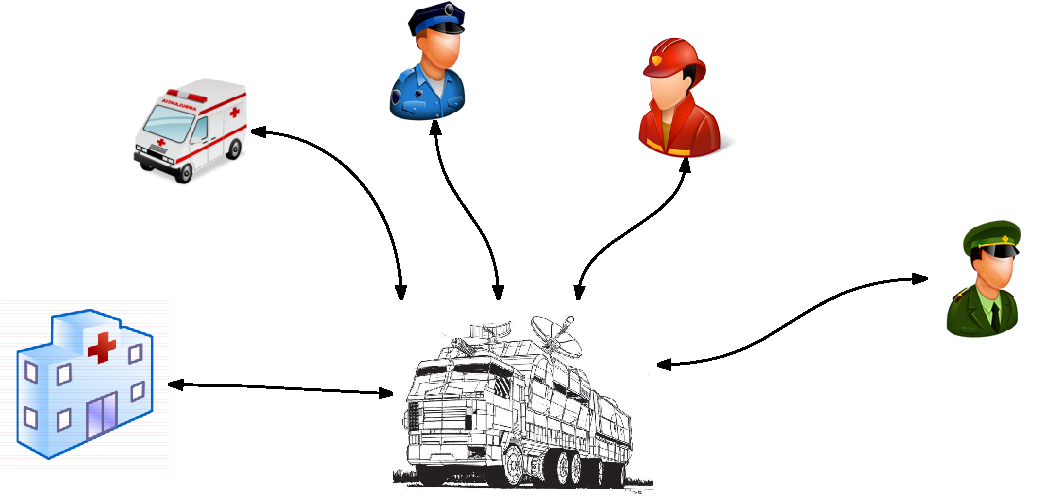
\includegraphics[width=0.95\textwidth]
{billeder/system_overview.pdf}
\caption{System Overview.}
\label{fig:system_overview}
\end{figure}


